Two AlphaSense O3 sensors were tested against the EPA reference.  The first sensor was 2.5 years old at the time of installation,  which ran for 38 days (from 4/15 to 5/23 2016 with one 40 minute service interruption).  The second sensor was 2 months old at the time of installation, and ran for 21 days (from 5/23 - 6/13 2016).  Our first test gave 55,589 minute-resolution samples to compare; our second test gave 30,150 samples.

Age is an important distinction between the two sensors, which makes this an interesting comparison.  Additionally, while the first O3 sensor was only calibrated for O3 measurement, the second sensor was calibrated as an O3+NO2 sensor (to be used in conjunction with the NO2 sensor on the board).  This presents a different calibration process- while the second sensor should be more accurate (as both are cross-sensitive to NO2), it depends on the accuracy of the NO2 characterization. The second sensor has a more complicated calibration equation, and thus introduces more opportunity for drift in the calibration process.

\subsection{Pre-processing}

The raw data for the O3 sensors is some of the most convincing we've recorded with a sensor at this price-point.  The calibrated values for both sensors track the real values quite well, and even capture a few transients.  A small sample of the datasheet-calibrated values is shown in Figure \ref{fig:as1_o3_raw_zoomed}-- for a look at all of the raw data, please check Appendix D.  

The preprocessing step followed similar guiding principles as the other AlphaSense sensors.  The final results for both sensors can be seen in Figure \ref{fig:as_o3_with_7p5_accuracy_zoomed} (Sensor \#1 on the left of the dotted line and Sensor \#2 on the right).  

\begin{figure}[htb]
 	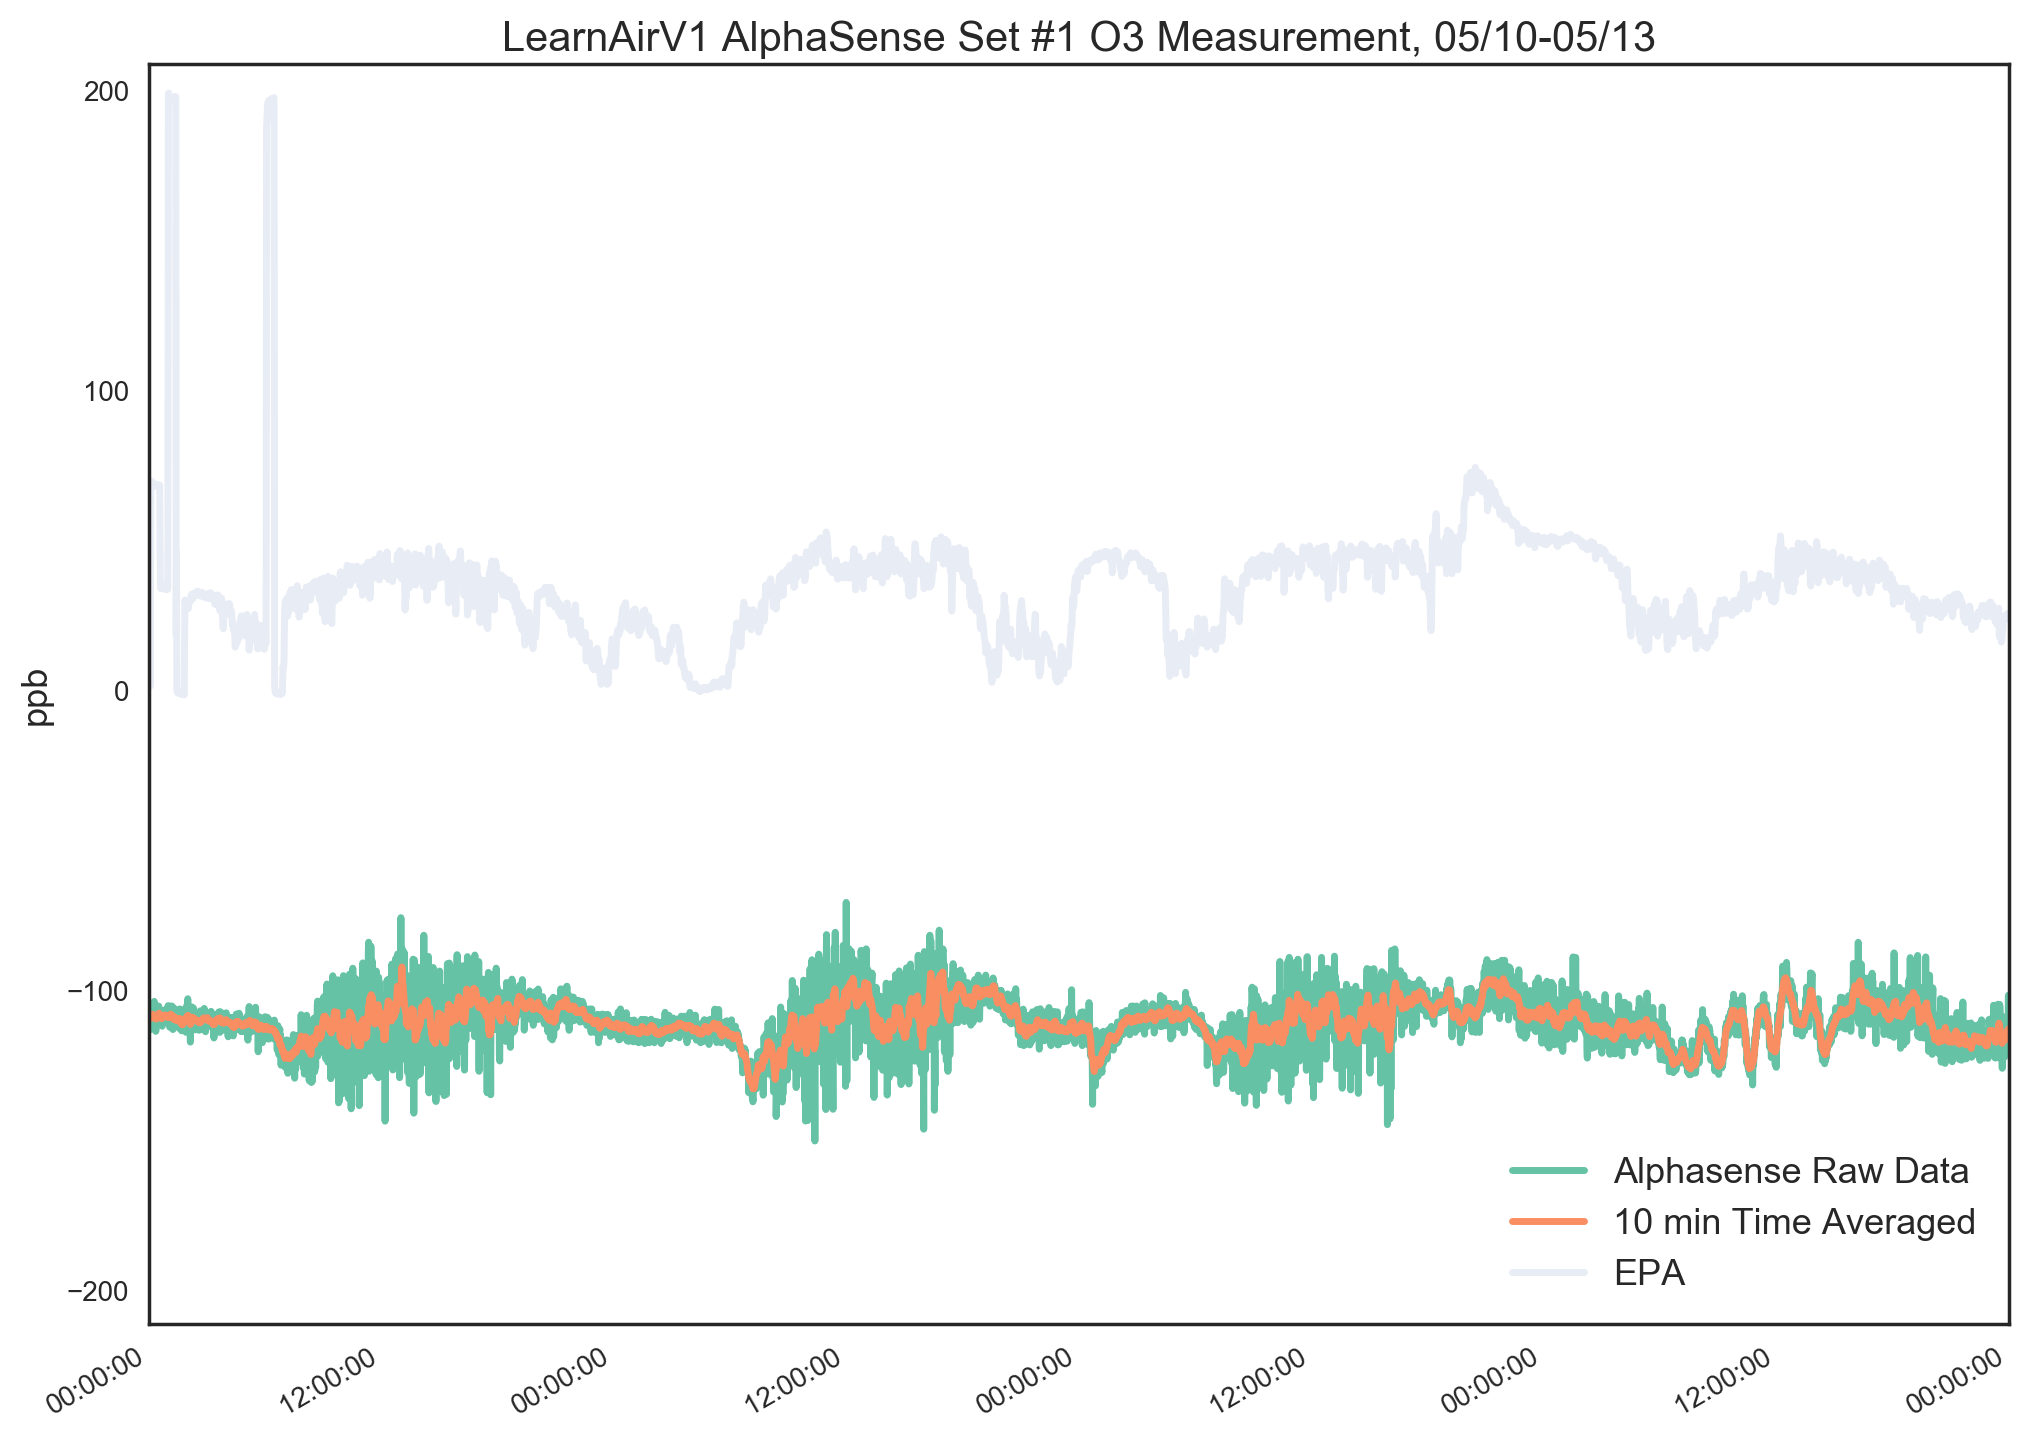
\includegraphics[width=\textwidth]{figs/as1_o3_raw_zoomed}               
 	 \caption{AlphaSense O3 Sensor #1 Raw Data Zoomed}
  	\label{fig:as1_o3_raw_zoomed}
\end{figure}


\subsection{Machine Learning}

O3 varies the least of the pollutants we measured, and our 15\% tolerance of full scale works out to be $\pm$15 ppb.  This is extremely tight-- the analog board is only rated for $\pm$10.  The great thing is that a little less than half of our readings actually fall into that very strict tolerance.  It may, however, be unrealistic to demand this level of precision from this sensor.


\begin{figure}[htb]
 	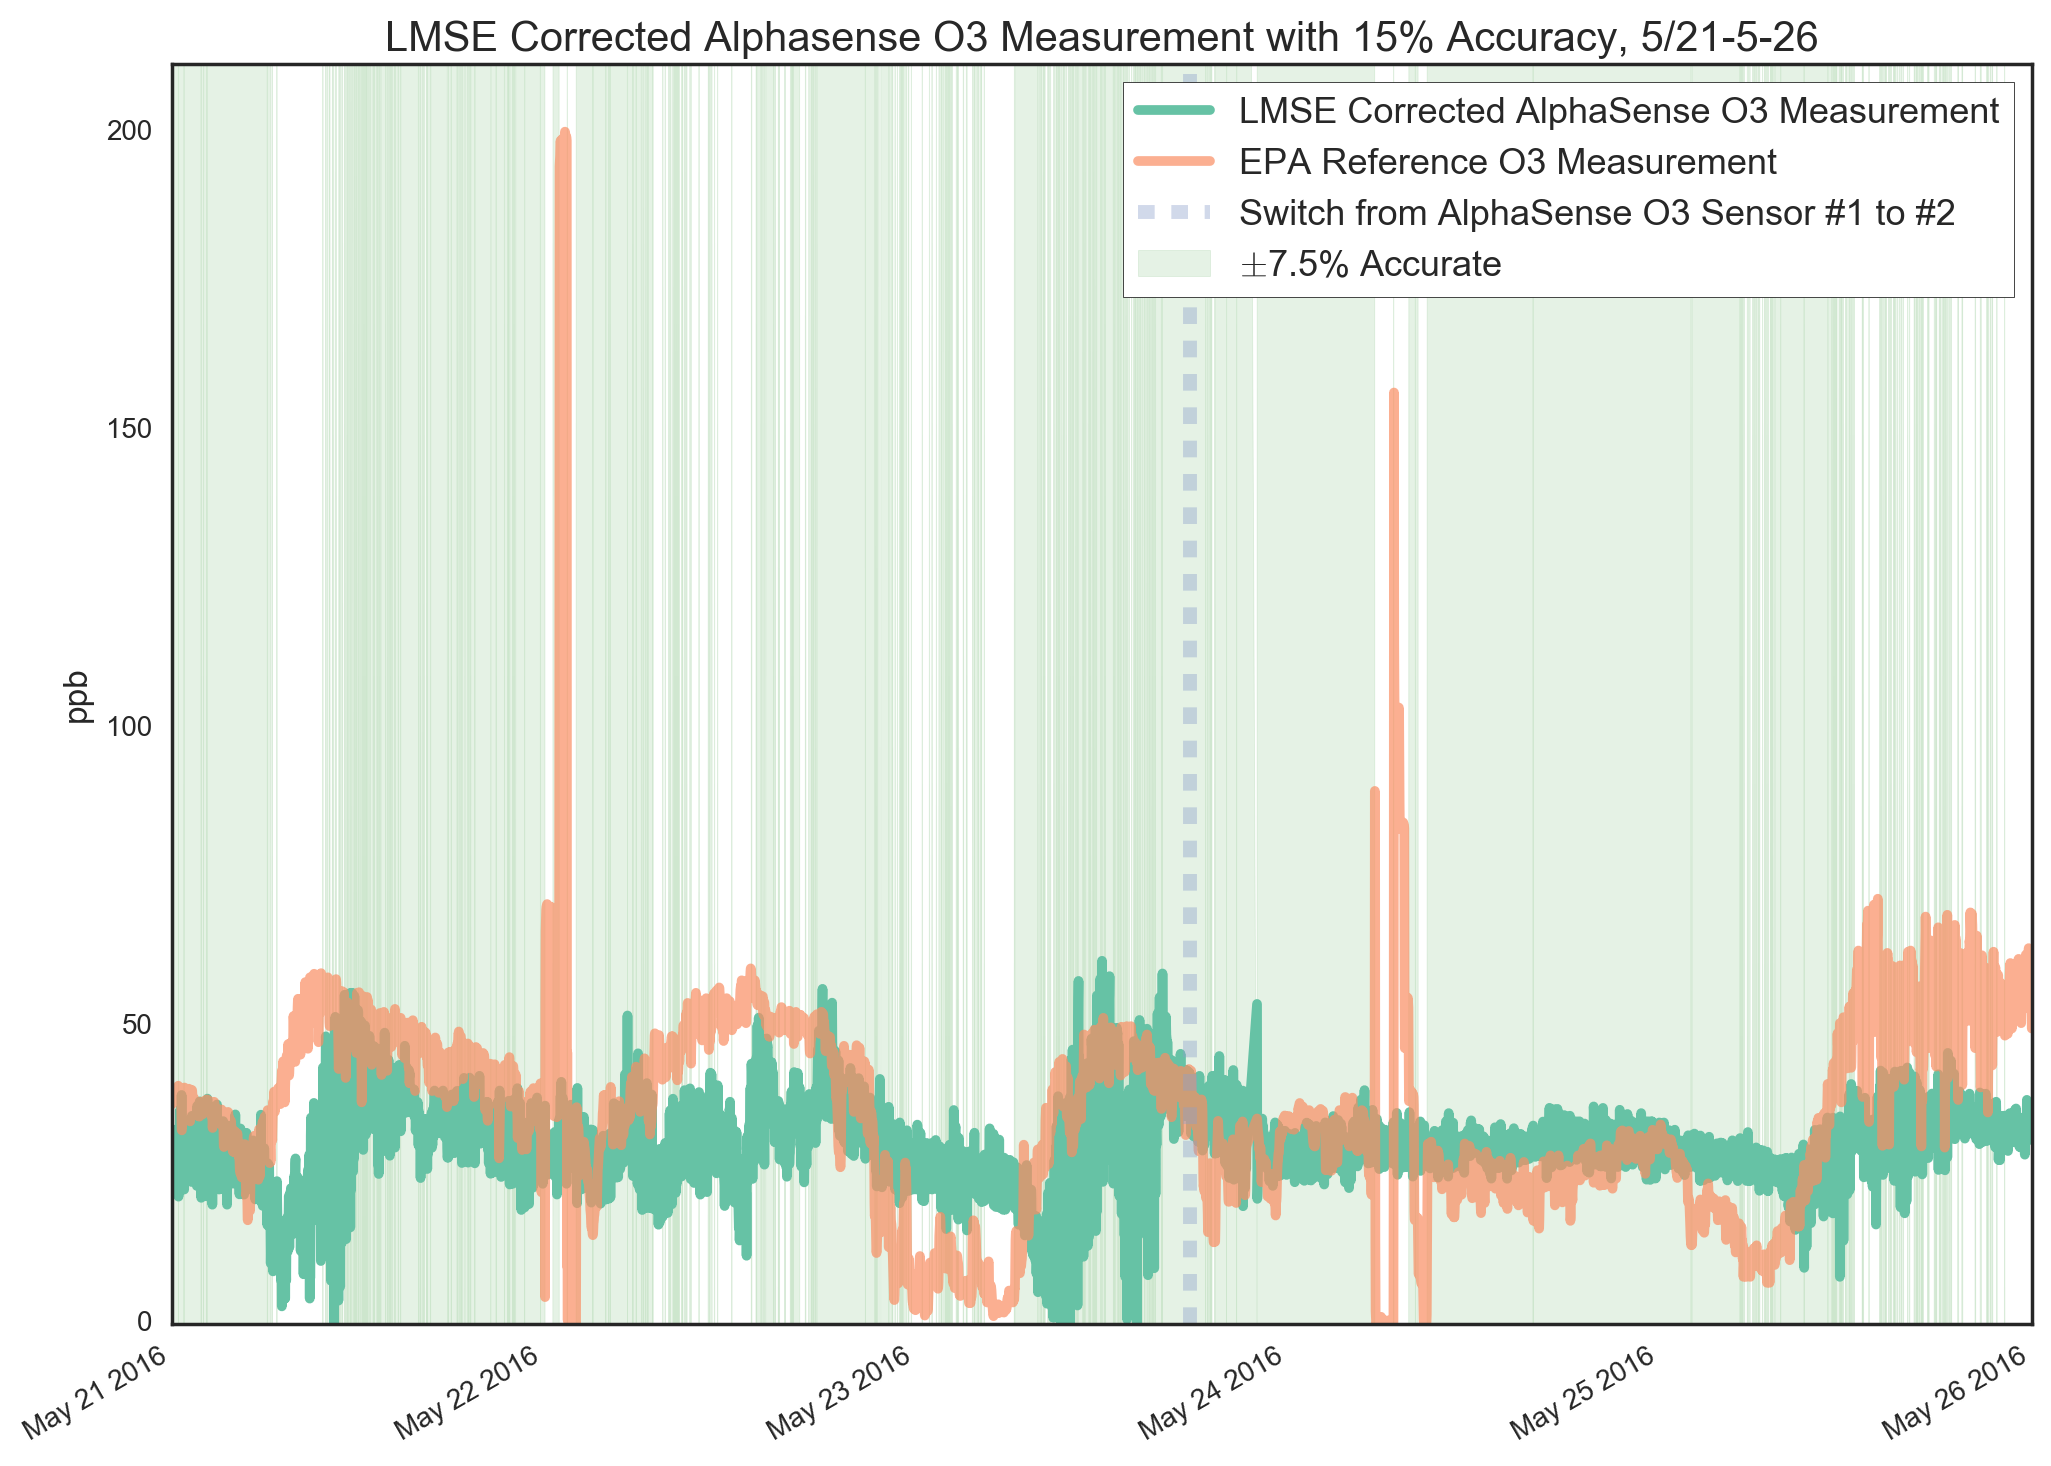
\includegraphics[width=\textwidth]{figs/as_o3_with_5_accuracy_zoomed}               
 	 \caption{AlphaSense O3 Sensor #1 and #2 with 15\% Accuracy Threshold}
  	\label{fig:as_o3_with_15_accuracy_zoomed}
\end{figure}


Our two fold search of the parameter space for both old and new O3 sensor gave an L1 penalty, and C values of 10 and 1000 respectively.  As we can see from Tables \ref{tab:as1_o3_error_rates} and \ref{tab:as2_o3_error_rates}, the errors levels we get when attempting to predict at this tolerance level are pretty extreme.  The confusion matrix and ROC curves back up that assumption.

\begin{table}
\centering
\begin{tabular}{|c|c|c|c|c|}
\toprule
\multicolumn{5}{|c|}{Error Rates for O3 Sensor #1 with Logistic Regression} \\
&\multicolumn{2}{|c|}{all features} & \multicolumn{2}{|c|}{top 15 features} \\
&shuffled & chunked & shuffled & chunked \\
avg & 0.33 & 0.43 & 0.37 & 0.41 \\
min & 0.32 & 0.37 & 0.36 & 0.36 \\
max & 0.33 & 0.52 & 0.37 & 0.52 \\
\bottomrule
\end{tabular}
\label{tab:as1_o3_error_rates}
\caption{Error Rates for Predicting O3 Sensor #1 Accuracy with Logistic Regression}
\end{table}

\begin{table}
\centering
\begin{tabular}{|c|c|c|c|c|}
\toprule
\multicolumn{5}{|c|}{Error Rates for O3 Sensor #2 with Logistic Regression} \\
&\multicolumn{2}{|c|}{all features} & \multicolumn{2}{|c|}{top 15 features} \\
&shuffled & chunked & shuffled & chunked \\
avg & 0.26 & 0.46 & 0.32 & 0.40 \\
min & 0.24 & 0.37 & 0.32 & 0.35 \\
max & 0.26 & 0.54 & 0.33 & 0.49 \\
\bottomrule
\end{tabular}
\label{tab:as2_o3_error_rates}
\caption{Error Rates for Predicting O3 Sensor #2 Accuracy with Logistic Regression}
\end{table}

The newer sensor appears to be more predictable, even with less data-- this may (again) be due to slightly more stable weather toward the end of the test.  Both sensors have strong trends between shuffled and chunked validation techniques, especially given the ambitious tolerance.  They are also surprising resilient to feature set reduction.

As a next step, it would be useful to increase the tolerance to a more reasonable level and re-train our model for prediction.  The quality of the readings suggests there is some very trustworthy and useful information to be had with this sensor.

\begin{margintable}
\centering
\offinterlineskip
\hspace*{-5cm}\raisebox{-4cm}[0pt][0pt]{\rotatebox[origin=c]{90}{\parbox[c][0pt][c]{3cm}{\textbf{Actual Values}\\[20pt]}}}\par
\hspace{.3cm}\MyHBox[\marginparwidth]{Predicted Values}\par
\vspace{-.5cm}
\hspace*{1cm}\MyHBox{0}\MyHBox{1}\par
\MyTBox{0}{4308.2}{1730.2}
\vspace{-.35cm}\MyTBox{1}{1931.8}{3147.6}\raisebox{-1cm}
}
\label{tab:as1_o3_confusion}
\caption{AlphaSense O3 Sensor #1 Confusion Matrix w/Shuffled K-Fold}
\end{margintable}



\begin{margintable}
\centering
\offinterlineskip
\hspace*{-5cm}\raisebox{-4cm}[0pt][0pt]{\rotatebox[origin=c]{90}{\parbox[c][0pt][c]{3cm}{\textbf{Actual Values}\\[20pt]}}}\par
\hspace{.3cm}\MyHBox[\marginparwidth]{Predicted Values}\par
\vspace{-.5cm}
\hspace*{1cm}\MyHBox{0}\MyHBox{1}\par
\MyTBox{0}{2439.6}{747.4}
\vspace{-.35cm}\MyTBox{1}{792.2}{2050.8}\raisebox{-1cm}
}
\label{tab:as2_o3_confusion}
\caption{AlphaSense O3 Sensor #2 Confusion Matrix w/Shuffled K-Fold}
\end{margintable}



\begin{figure}[htb]
 	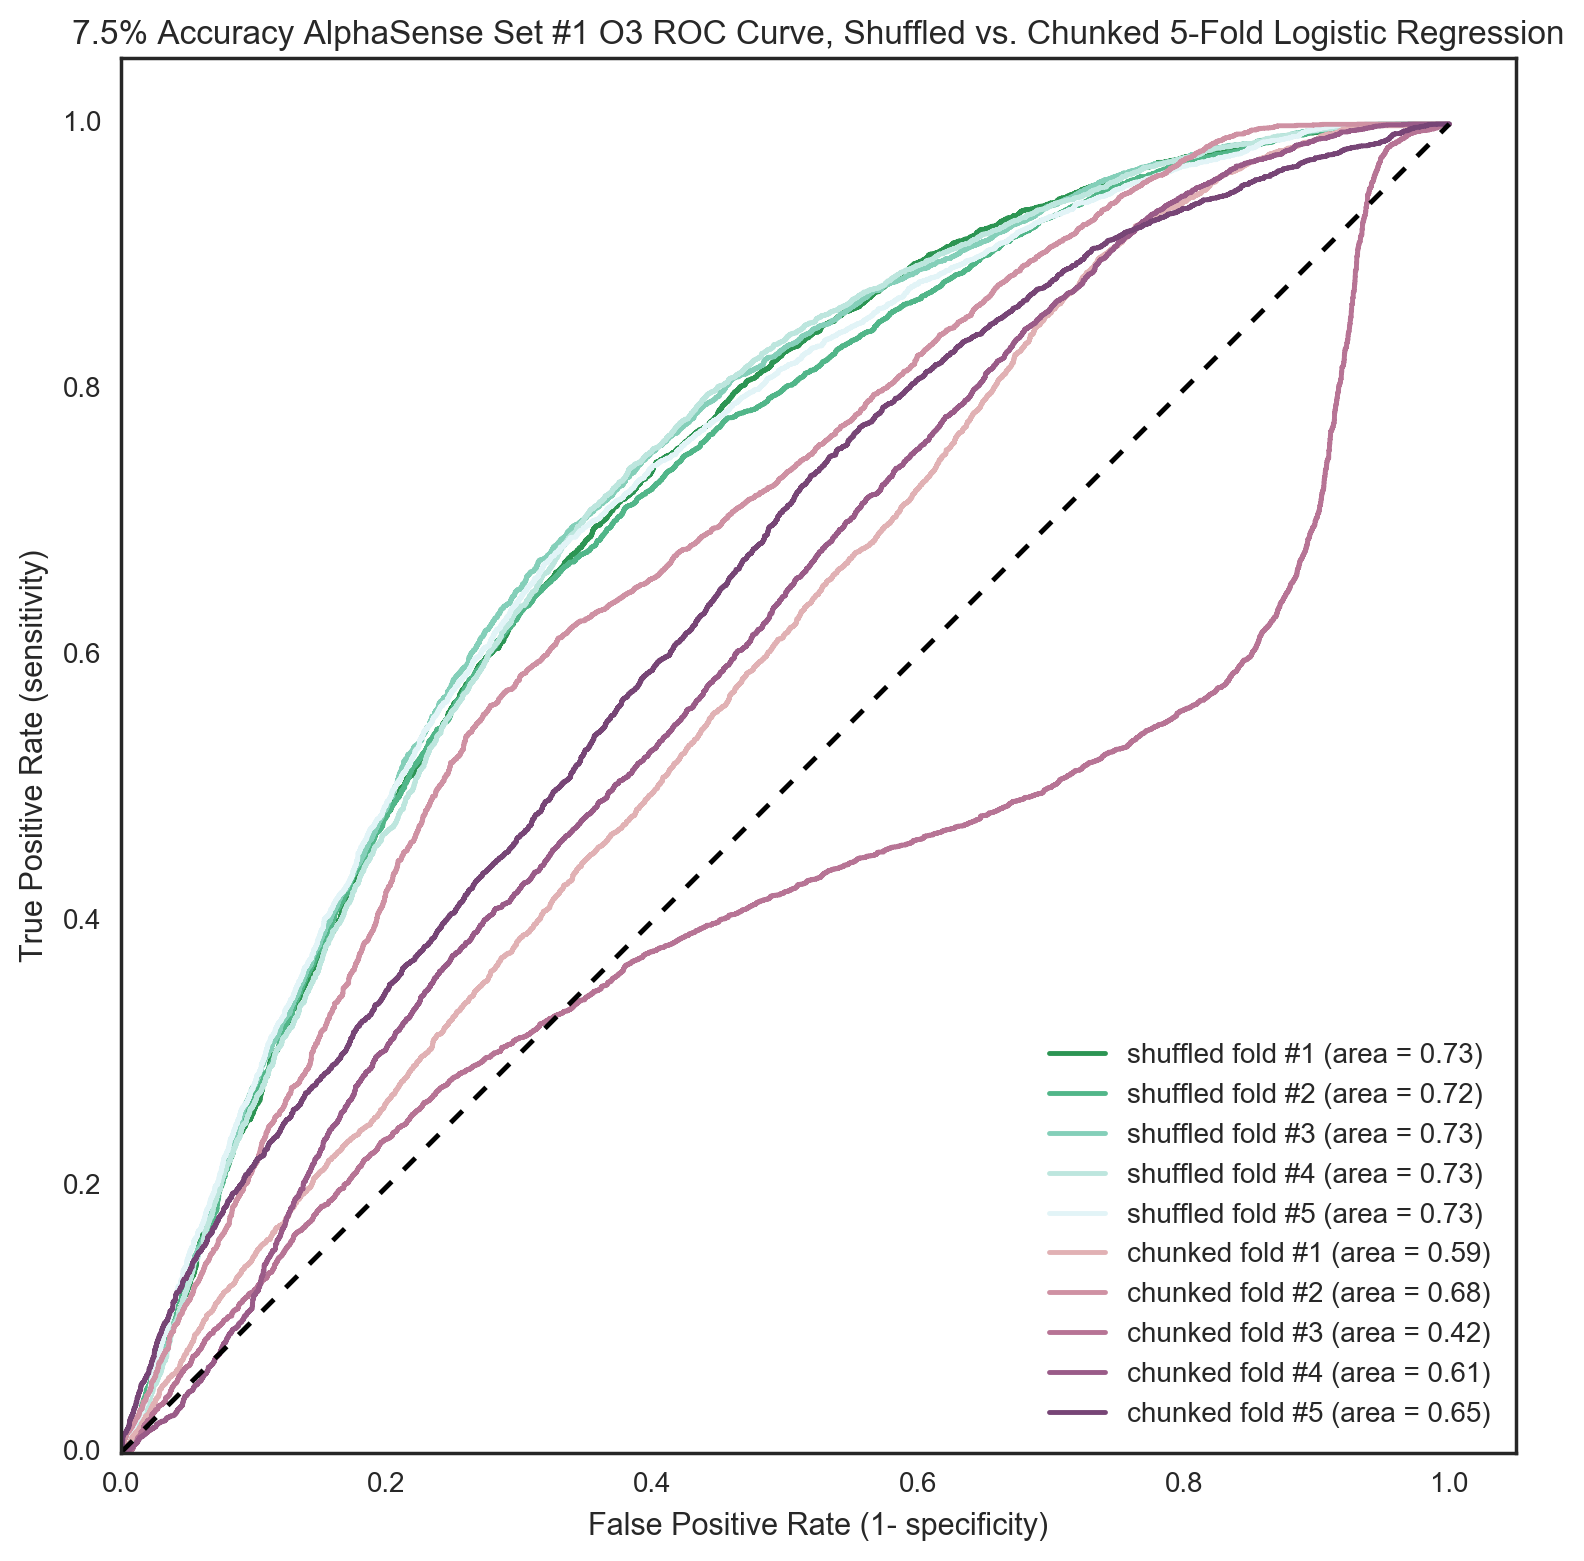
\includegraphics[width=\textwidth-1cm]{figs/as1_o3_7p5_roc}               
 	 \caption{AlphaSense O3 Sensor #1 ROC Curve}
  	\label{fig:as1_o3_7p5_roc}
\end{figure}


\begin{figure}[htb]
 	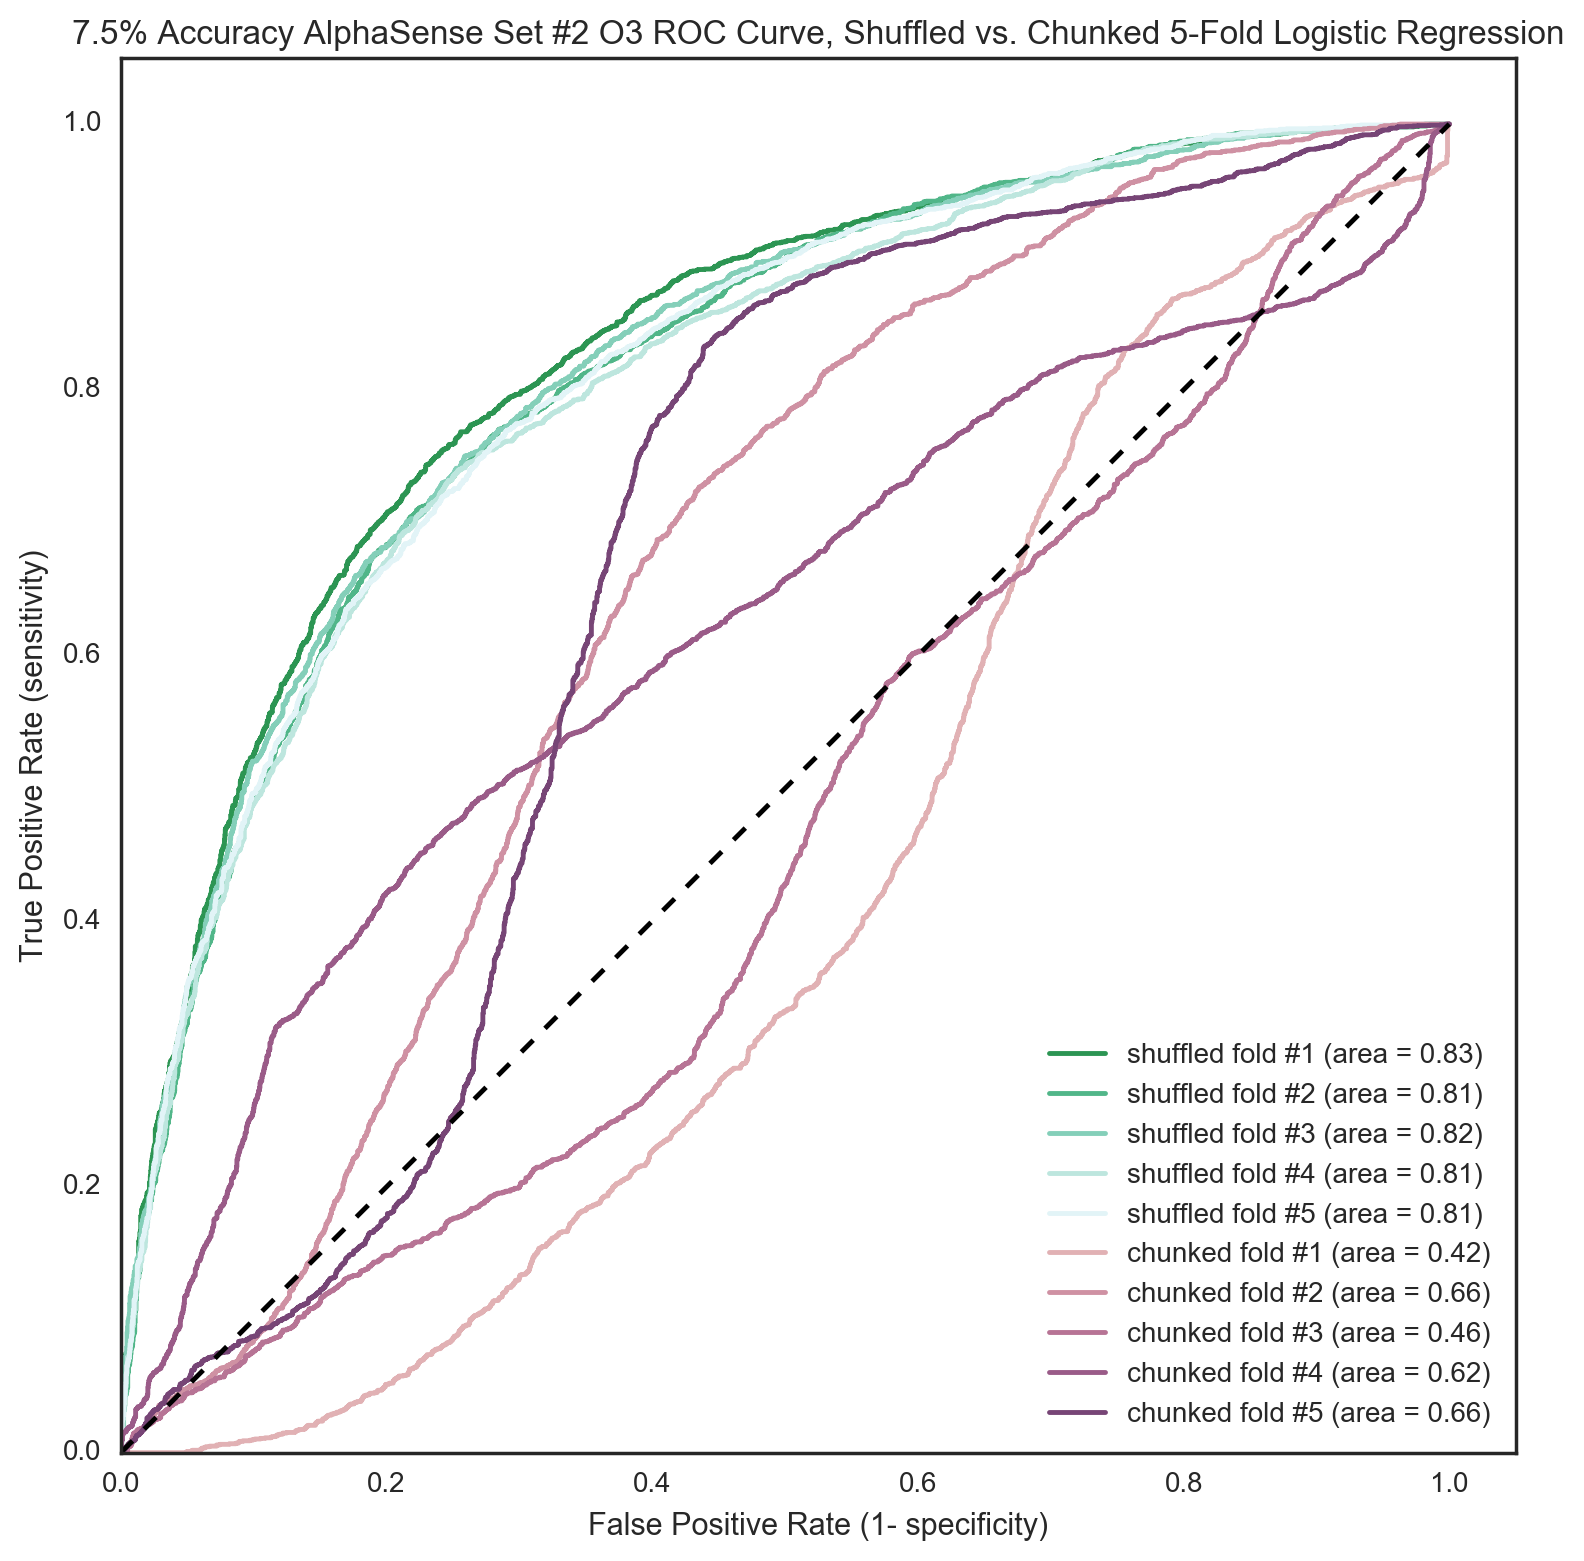
\includegraphics[width=\textwidth-1cm]{figs/as2_o3_7p5_roc}               
 	 \caption{AlphaSense O3 Sensor #2 ROC Curve}
  	\label{fig:as2_o3_7p5_roc}
\end{figure}


\begin{table}
\centering
\small
\begin{tabular}{lllllllll}
\\
\\
\toprule
     & Corr. & Lasso & Lin Reg & RF   & RFE  & Ridge & Stability & Mean \\
\midrule
alphaS1\_work                                  & 0.32  & 1     & 0          & 1    & 0.44 & 0.14  & 0.94      & 0.55 \\
as\_h2s                                        & 0.55  & 0.84  & 0          & 0.08 & 0.96 & 0.01  & 0.63      & 0.44 \\
avg\_1440\_lmse\_scaled\_sharpDust             & 0.22  & 0     & 0          & 0.08 & 0.52 & 1     & 1         & 0.4  \\
avg\_720\_bkcarbon                             & 1     & 0     & 0          & 0.24 & 0.54 & 0.27  & 0.59      & 0.38 \\
bkcarbon                                       & 0.97  & 0     & 0          & 0.18 & 0.27 & 0.24  & 0.77      & 0.35 \\
alphaS3\_aux                                   & 0.68  & 0     & 0          & 0.04 & 0.97 & 0.02  & 0.67      & 0.34 \\
forecastio\_windSpeed                          & 0.62  & 0.5   & 0          & 0.07 & 0.29 & 0.03  & 0.75      & 0.32 \\
Solar Panel ( V)                               & 0.17  & 0     & 1          & 0    & 0.98 & 0     & 0         & 0.31 \\
avg\_10\_as\_o3                                & 0.19  & 0.35  & 0          & 0.05 & 0.51 & 0.29  & 0.76      & 0.31 \\
Nitrogen Dioxide ( kOhm)                       & 0.59  & 0.04  & 0          & 0.04 & 0.74 & 0     & 0.67      & 0.3  \\
lmse\_sck\_no2                                 & 0.59  & 0     & 0          & 0.04 & 0.74 & 0     & 0.73      & 0.3  \\
avg\_60\_bkcarbon                              & 0.84  & 0     & 0          & 0.19 & 0.49 & 0.02  & 0.59      & 0.3  \\
derivative\_avg\_1440\_bkcarbon                & 0.19  & 0     & 0          & 0.07 & 0.63 & 0.18  & 1         & 0.3  \\
avg\_1440\_bkcarbon                            & 0.78  & 0     & 0          & 0.25 & 0.53 & 0.36  & 0.01      & 0.28 \\
derivative\_avg\_720\_bkcarbon                 & 0.08  & 0     & 0          & 0.05 & 0.61 & 0.21  & 1         & 0.28 \\
daily\_avg\_forecastio\_humidity               & 0.08  & 0     & 0          & 0.28 & 0.55 & 0.95  & 0.01      & 0.27 \\
avg\_15\_derivative\_avg\_15\_as\_temperature  & 0.3   & 0     & 0          & 0.07 & 0.49 & 0.29  & 0.65      & 0.26 \\
alphaS1\_aux                                   & 0.01  & 0.93  & 0          & 0.06 & 0.45 & 0.13  & 0.17      & 0.25 \\
avg\_60\_forecastio\_temperature\_c            & 0.42  & 0     & 0.01       & 0.07 & 0.76 & 0.01  & 0.48      & 0.25 \\
humidity\_box\_differential                    & 0.15  & 0     & 0.03       & 0.1  & 1    & 0.08  & 0.42      & 0.25 \\
avg\_10\_lmse\_calib\_as\_o3                   & 0.19  & 0     & 0          & 0.04 & 0.51 & 0.29  & 0.7       & 0.25 \\
derivative\_avg\_60\_bkcarbon                  & 0.11  & 0     & 0          & 0.05 & 0.58 & 0.42  & 0.56      & 0.25 \\
derivative\_avg\_1440\_lmse\_scaled\_sharpDust & 0.01  & 0     & 0          & 0.06 & 0.62 & 0.07  & 1         & 0.25 \\
as\_o3                                         & 0.04  & 0     & 0          & 0.76 & 0.79 & 0.01  & 0.07      & 0.24 \\
\bottomrule
\end{tabular}
\label{tab:as1_o3_top_features}
\caption{Top Features for Predicting AlphaSense O3 Sensor #1}
\end{table}



\begin{table}[!htb]
\centering
\small
\begin{tabular}{lllllllll}
\\
\\
\toprule
     & Corr. & Lasso & Lin Reg & RF   & RFE  & Ridge & Stability & Mean \\
\midrule
avg\_1440\_as\_co                             & 1     & 0.12  & 0          & 0.58 & 0.08 & 0     & 1         & 0.4  \\
daily\_avg\_sck\_humidity                     & 0.71  & 0     & 0          & 0.07 & 0.57 & 1     & 0.36      & 0.39 \\
avg\_1440\_bkcarbon                           & 0.66  & 0     & 0          & 1    & 0.48 & 0.33  & 0.01      & 0.35 \\
avg\_60\_bkcarbon                             & 0.79  & 0     & 0          & 0.38 & 0.35 & 0.06  & 0.8       & 0.34 \\
forecastio\_pressure                          & 0.27  & 0.82  & 0          & 0.1  & 0.33 & 0.04  & 0.75      & 0.33 \\
avg\_60\_forecastio\_apparentTemperature      & 0.17  & 1     & 0          & 0.07 & 0.4  & 0.09  & 0.57      & 0.33 \\
avg\_15\_derivative\_sck\_temperature         & 0.03  & 0     & 0          & 0.04 & 0.57 & 0.45  & 1         & 0.3  \\
bkcarbon                                      & 0.73  & 0     & 0          & 0.14 & 0.47 & 0.04  & 0.66      & 0.29 \\
Solar Panel ( V)                              & 0.1   & 0     & 1          & 0    & 0.86 & 0     & 0         & 0.28 \\
avg\_720\_bkcarbon                            & 0.76  & 0     & 0          & 0.38 & 0.45 & 0.23  & 0.12      & 0.28 \\
derivative\_avg\_1440\_lmse\_calib\_as\_co    & 0.16  & 0     & 0          & 0.08 & 0.51 & 0.14  & 1         & 0.27 \\
daily\_avg\_as\_temperature                   & 0.79  & 0     & 0          & 0.19 & 0.43 & 0.11  & 0.31      & 0.26 \\
lmse\_avg\_30\_scaled\_arduino\_ws            & 0.34  & 0.06  & 0          & 0.04 & 0.94 & 0.01  & 0.4       & 0.26 \\
avg\_1440\_lmse\_scaled\_sharpDust            & 0.05  & 0     & 0          & 0.1  & 0.53 & 0.39  & 0.77      & 0.26 \\
derivative\_avg\_720\_lmse\_scaled\_sharpDust & 0.1   & 0     & 0          & 0.08 & 0.61 & 0.05  & 1         & 0.26 \\
alphaS1\_aux                                  & 0     & 0     & 0.03       & 0.04 & 0.69 & 0.02  & 1         & 0.25 \\
avg\_30\_scaled\_arduino\_ws                  & 0.34  & 0     & 0.01       & 0.04 & 0.95 & 0     & 0.41      & 0.25 \\
derivative\_avg\_1440\_bkcarbon               & 0.09  & 0     & 0          & 0.06 & 0.61 & 0.01  & 1         & 0.25 \\
forecastio\_cloudCover                        & 0.23  & 0     & 0          & 0.16 & 0.49 & 0.01  & 0.64      & 0.22 \\
forecastio\_clear-day                         & 0.01  & 0     & 0.03       & 0    & 0.89 & 0.02  & 0.56      & 0.22 \\
avg\_60\_forecastio\_pressure                 & 0.28  & 0     & 0          & 0.2  & 0.33 & 0.03  & 0.72      & 0.22 \\
Nitrogen Dioxide ( kOhm)                      & 0.1   & 0.13  & 0          & 0.04 & 0.78 & 0     & 0.41      & 0.21 \\
forecastio\_temperature\_c                    & 0.17  & 0     & 0.01       & 0.27 & 0.87 & 0.05  & 0.06      & 0.2  \\
avg\_60\_as\_no2                              & 0.03  & 0.04  & 0          & 0.09 & 0.77 & 0     & 0.47      & 0.2 \\
\bottomrule
\end{tabular}
\label{tab:as2_o3_top_features}
\caption{Top Features for Predicting AlphaSense O3 Sensor #2}
\end{table}



